\documentclass[12pt,letterpaper]{article}

\usepackage[spanish]{babel}
\usepackage[margin=2.5cm]{geometry} 
\usepackage{listings}
\usepackage{graphicx}
\usepackage{xcolor}
\usepackage{float} 

% Configuración de estilos para el bloque de código SQL
\definecolor{codegreen}{rgb}{0,0.6,0}
\definecolor{codegray}{rgb}{0.5,0.5,0.5}
\definecolor{codepurple}{rgb}{0.58,0,0.82}
\definecolor{backcolour}{rgb}{0.95,0.95,0.92}

\lstdefinestyle{mystyle}{
    backgroundcolor=\color{backcolour},   
    commentstyle=\color{codegreen},
    keywordstyle=\color{magenta},
    numberstyle=\tiny\color{codegray},
    stringstyle=\color{codepurple},
    basicstyle=\ttfamily\scriptsize, 
    breakatwhitespace=false,         
    breaklines=true,                 
    captionpos=b,                    
    keepspaces=true,                 
    numbers=left,                    
    numbersep=5pt,                  
    showspaces=false,                
    showstringspaces=false,
    showtabs=false,                  
    tabsize=2,
    literate={á}{{\'a}}1 {é}{{\'e}}1 {í}{{\'i}}1 {ó}{{\'o}}1 {ú}{{\'u}}1
             {Á}{{\'A}}1 {É}{{\'E}}1 {Í}{{\'I}}1 {Ó}{{\'O}}1 {Ú}{{\'U}}1
             {ñ}{{\~n}}1 {Ñ}{{\~N}}1 {¿}{{?`}}1 {¡}{{!`}}1
}
\lstset{style=mystyle}

\renewcommand{\lstlistingname}{Código}
\renewcommand{\lstlistlistingname}{Lista de códigos}

\author{Sergio Ezequiel De Luis Sanchez}
\title{Reporte de una base de datos}
\date{\today}

\begin{document}
\maketitle
\tableofcontents
\listoffigures
\listoftables
\lstlistoflistings

\vspace{1cm}

\section{Introducción}
Se nos ha encomendado realizar ingeniería inversa y, posterior, análisis de un conjunto de archivos que comprenden la definición estructural y lógica de la base de datos de un sistema ``Legacy''. Con la finalidad de practicar e integrar todo lo aprendido hasta el momento.

\section{Descripción del problema}
Una institución educativa necesita modernizar y centralizar su control administrativo y académico. Actualmente requiere un sistema de bases de datos relacional que gestione de manera eficiente la información de sus departamentos, el personal docente, la oferta de cursos, las inscripciones de los estudiantes, así como la asignación de espacios físicos y horarios de clase.

\section{Análisis}
El dominio de la institución se organiza conceptualmente a través de \textbf{departamentos}, los cuales identifican las diferentes áreas de la escuela. Cada departamento agrupa a varios \textbf{profesores}, de quienes se guarda su información personal y de contacto. 

Cada profesor tiene a su cargo la impartición de distintos \textbf{cursos}, los cuales tienen un nombre específico y otorgan una cantidad determinada de créditos académicos. Por otro lado, la escuela registra a sus \textbf{estudiantes} con sus datos básicos y fecha de nacimiento. Los estudiantes se matriculan en los cursos mediante \textbf{inscripciones}, registrando la fecha exacta del trámite. A través de estas inscripciones, el sistema vincula y registra las \textbf{notas} o calificaciones obtenidas por el alumno en dicha materia.

Para la logística de las sesiones, la escuela cuenta con \textbf{aulas} que poseen una capacidad máxima definida. Las clases se estructuran a través de \textbf{horarios}, los cuales vinculan de manera precisa un curso con un aula específica, detallando el día de la semana en que se imparte, junto con la hora de inicio y fin.

Para la documentación de esta arquitectura de datos, se omitió la escritura manual de los scripts en favor de un enfoque visual y automatizado. Se aplicó un proceso de ingeniería inversa (Reverse Engineering) directamente sobre el script SQL de creación de la base de datos. Este procedimiento permitió a la herramienta de modelado leer e interpretar las tablas, atributos, tipos de datos, llaves primarias y las restricciones de llaves foráneas, garantizando una correspondencia exacta con el sistema analizado.

\subsection{Estructura detallada de la base de datos}

A continuación se detalla la composición de cada una de las entidades del sistema, así como las relaciones establecidas mediante llaves foráneas.

\begin{table}[H]
    \centering
    \begin{tabular}{|l|l|}
    \hline
    \textbf{Columna} & \textbf{Tipo de Dato} \\ \hline
    id & INT (PK) \\ 
    nombre & VARCHAR(100) \\ \hline
    \end{tabular}
    \caption{Entidad: departamentos}
\end{table}

\begin{table}[H]
    \centering
    \begin{tabular}{|l|l|}
    \hline
    \textbf{Columna} & \textbf{Tipo de Dato} \\ \hline
    id & INT (PK) \\ 
    nombre & VARCHAR(100) \\ 
    apellido & VARCHAR(100) \\ 
    email & VARCHAR(100) \\ 
    id\_departamento & INT (FK) \\ \hline
    \end{tabular}
    \caption{Entidad: profesores}
\end{table}

\begin{table}[H]
    \centering
    \begin{tabular}{|l|l|}
    \hline
    \textbf{Columna} & \textbf{Tipo de Dato} \\ \hline
    id & INT (PK) \\ 
    nombre & VARCHAR(100) \\ 
    creditos & INT \\ 
    id\_profesor & INT (FK) \\ \hline
    \end{tabular}
    \caption{Entidad: cursos}
\end{table}

\begin{table}[H]
    \centering
    \begin{tabular}{|l|l|}
    \hline
    \textbf{Columna} & \textbf{Tipo de Dato} \\ \hline
    id & INT (PK) \\ 
    nombre & VARCHAR(100) \\ 
    apellido & VARCHAR(100) \\ 
    email & VARCHAR(100) \\ 
    fecha\_nacimiento & DATE \\ \hline
    \end{tabular}
    \caption{Entidad: estudiantes}
\end{table}

\begin{table}[H]
    \centering
    \begin{tabular}{|l|l|}
    \hline
    \textbf{Columna} & \textbf{Tipo de Dato} \\ \hline
    id & INT (PK) \\ 
    id\_estudiante & INT (FK) \\ 
    id\_curso & INT (FK) \\ 
    fecha\_inscripcion & DATE \\ \hline
    \end{tabular}
    \caption{Entidad: inscripciones}
\end{table}

\begin{table}[H]
    \centering
    \begin{tabular}{|l|l|}
    \hline
    \textbf{Columna} & \textbf{Tipo de Dato} \\ \hline
    id & INT (PK) \\ 
    nombre & VARCHAR(50) \\ 
    capacidad & INT \\ \hline
    \end{tabular}
    \caption{Entidad: aulas}
\end{table}

\begin{table}[H]
    \centering
    \begin{tabular}{|l|l|}
    \hline
    \textbf{Columna} & \textbf{Tipo de Dato} \\ \hline
    id & INT (PK) \\ 
    id\_curso & INT (FK) \\ 
    id\_aula & INT (FK) \\ 
    dia\_semana & VARCHAR(15) \\ 
    hora\_inicio & TIME \\ 
    hora\_fin & TIME \\ \hline
    \end{tabular}
    \caption{Entidad: horarios}
\end{table}

\begin{table}[H]
    \centering
    \begin{tabular}{|l|l|}
    \hline
    \textbf{Columna} & \textbf{Tipo de Dato} \\ \hline
    id & INT (PK) \\ 
    id\_inscripcion & INT (FK) \\ 
    nota & DECIMAL(4,2) \\ \hline
    \end{tabular}
    \caption{Entidad: notas}
\end{table}

\begin{table}[H]
\centering
\begin{tabular}{lll}
  \hline
  \textbf{Tabla origen} & \textbf{Columna FK} & \textbf{Tabla destino} \\
  \hline
  \texttt{profesores}    & \texttt{id\_departamento}  & \texttt{departamentos} \\
  \texttt{cursos}        & \texttt{id\_profesor}      & \texttt{profesores}    \\
  \texttt{inscripciones} & \texttt{id\_estudiante}    & \texttt{estudiantes}   \\
  \texttt{inscripciones} & \texttt{id\_curso}         & \texttt{cursos}        \\
  \texttt{horarios}      & \texttt{id\_curso}         & \texttt{cursos}        \\
  \texttt{horarios}      & \texttt{id\_aula}          & \texttt{aulas}         \\
  \texttt{notas}         & \texttt{id\_inscripcion}   & \texttt{inscripciones} \\
  \hline
\end{tabular}
\caption{Relaciones y dependencias entre tablas.}
\end{table}

\section{Diagramas y respuestas}

\begin{figure}[H] 
    \centering
    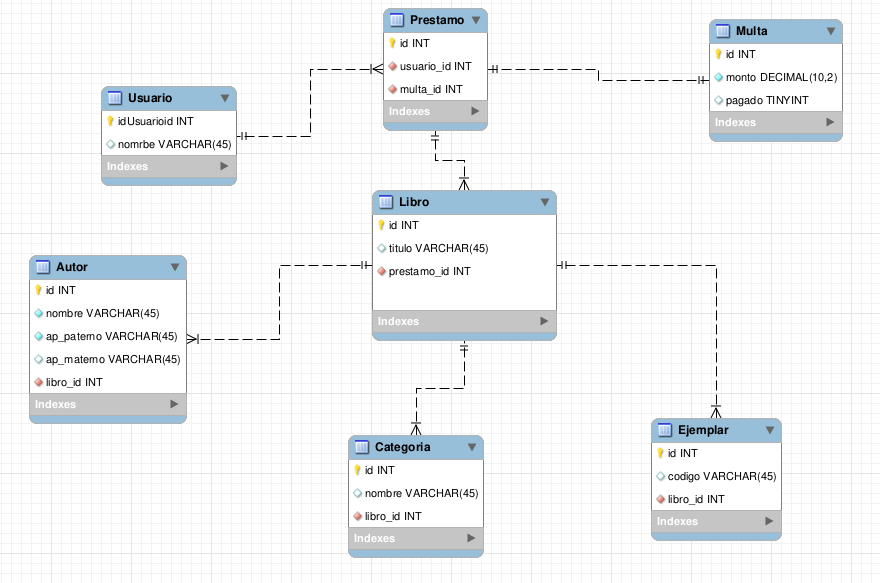
\includegraphics[width=\textwidth]{mer.png}
    \caption{Diagrama entidad-relación para el modelo de datos del Sistema Escolar, generado mediante ingeniería inversa.}\label{fig_der}
\end{figure}

Una vez interpretada la estructura física del esquema, se procedió al poblado inicial de las tablas para realizar las pruebas de validación pertinentes. El siguiente script detalla las inserciones de datos y transaccionales ejecutadas para simular el entorno escolar:

\begin{lstlisting}[language=SQL, frame=single, caption={Script de inserción de datos iniciales en la base de datos escolar}]
-- Insertar datos en Departamentos
INSERT INTO departamentos (nombre) VALUES 
('Matemáticas'), ('Ciencias'), ('Humanidades'), ('Ingeniería');

-- Insertar datos en Profesores
INSERT INTO profesores (nombre, apellido, email, id_departamento) VALUES
('Ana', 'Ramírez', 'ana.ramirez@escuela.edu', 1),
('Luis', 'González', 'luis.gonzalez@escuela.edu', 2),
('Clara', 'López', 'clara.lopez@escuela.edu', 3),
('Pedro', 'Martínez', 'pedro.martinez@escuela.edu', 4);

-- Insertar datos en Cursos
INSERT INTO cursos (nombre, creditos, id_profesor) VALUES
('Álgebra', 5, 1), ('Biología', 4, 2), ('Historia', 3, 3),
('Programación', 6, 4), ('Física', 4, 2), ('Ética', 2, 3);

-- Insertar datos en Estudiantes
INSERT INTO estudiantes (nombre, apellido, email, fecha_nacimiento) 
VALUES
('Juan', 'Pérez', 'juan.perez@correo.com', '2000-04-15'),
('María', 'Gómez', 'maria.gomez@correo.com', '2001-06-21'),
('Carlos', 'Sánchez', 'carlos.sanchez@correo.com', '1999-12-30'),
('Lucía', 'Díaz', 'lucia.diaz@correo.com', '2002-01-10');

-- Insertar datos en Inscripciones
INSERT INTO inscripciones (id_estudiante, id_curso, fecha_inscripcion) 
VALUES
(1, 1, '2024-01-15'), (1, 2, '2024-01-15'), (2, 1, '2024-01-20'),
(2, 3, '2024-01-21'), (3, 4, '2024-01-22'), (4, 5, '2024-01-23');

-- Insertar datos en Aulas
INSERT INTO aulas (nombre, capacidad) VALUES
('Aula 101', 30), ('Aula 102', 25),
('Laboratorio 1', 20), ('Sala Conferencias', 50);

-- Insertar datos en Horarios
INSERT INTO horarios (id_curso, id_aula, dia_semana, hora_inicio, hora_fin) 
VALUES
(1, 1, 'Lunes', '08:00:00', '10:00:00'),
(2, 2, 'Martes', '10:00:00', '12:00:00'),
(3, 4, 'Miércoles', '13:00:00', '15:00:00'),
(4, 3, 'Jueves', '09:00:00', '11:00:00'),
(5, 2, 'Viernes', '08:00:00', '10:00:00');

-- Insertar datos en Notas
INSERT INTO notas (id_inscripcion, nota) VALUES
(1, 8.5), (2, 9.0), (3, 7.5), (4, 6.8), (5, 9.2), (6, 7.0);
\end{lstlisting}

\subsection{Consultas}

Con la base de datos creada y con datos, se debe  responder un listado formulando las sentencias SQL de consulta, arrojando los siguientes resultados:

\begin{enumerate}
    \item ¿Cuáles son los estudiantes inscritos en el curso "Álgebra"?
\begin{lstlisting}[language=SQL, frame=single]
SELECT e.nombre, e.apellido 
FROM estudiantes e 
JOIN inscripciones i ON e.id = i.id_estudiante 
JOIN cursos c ON i.id_curso = c.id 
WHERE c.nombre = 'Álgebra';
\end{lstlisting}
    \begin{table}[H]
        \centering
        \begin{tabular}{|l|l|}
        \hline
        \textbf{nombre} & \textbf{apellido} \\ \hline
        Juan & Pérez \\ 
        María & Gómez \\ \hline
        \end{tabular}
    \end{table}

    \item ¿Qué cursos imparte el profesor Pedro Martínez?
\begin{lstlisting}[language=SQL, frame=single]
SELECT c.nombre AS Nombre_curso, 
concat(p.nombre, " ",p.apellido) as Nombre_profesor
FROM cursos c
inner JOIN profesores p ON c.id_profesor = p.id 
WHERE p.nombre = 'Pedro' AND p.apellido = 'Martínez';
\end{lstlisting}
    \begin{table}[H]
        \centering
        \begin{tabular}{|l|l|}
        \hline
        \textbf{Nombre\_curso} & \textbf{Nombre\_profesor} \\ \hline
        Programación & Pedro Martínez \\ \hline
        \end{tabular}
    \end{table}

    \item ¿Cuántos estudiantes están inscritos en cada curso?
\begin{lstlisting}[language=SQL, frame=single]
SELECT c.nombre, COUNT(i.id_estudiante) AS total_estudiantes 
FROM cursos c 
LEFT JOIN inscripciones i ON c.id = i.id_curso 
GROUP BY c.id, c.nombre;
\end{lstlisting}
    \begin{table}[H]
        \centering
        \begin{tabular}{|l|l|}
        \hline
        \textbf{nombre} & \textbf{total\_estudiantes} \\ \hline
        Álgebra & 2 \\ 
        Biología & 1 \\ 
        Historia & 1 \\ 
        Programación & 1 \\ 
        Física & 1 \\ 
        Ética & 0 \\ \hline
        \end{tabular}
    \end{table}

    \item ¿Cuál es el promedio de notas por curso?
\begin{lstlisting}[language=SQL, frame=single]
SELECT c.nombre, AVG(n.nota) AS promedio_notas 
FROM cursos c 
JOIN inscripciones i ON c.id = i.id_curso 
JOIN notas n ON i.id = n.id_inscripcion 
GROUP BY c.id, c.nombre;
\end{lstlisting}
    \begin{table}[H]
        \centering
        \begin{tabular}{|l|l|}
        \hline
        \textbf{nombre} & \textbf{promedio\_notas} \\ \hline
        Álgebra & 8.00 \\ 
        Biología & 9.00 \\ 
        Historia & 6.80 \\ 
        Programación & 9.20 \\ 
        Física & 7.00 \\ \hline
        \end{tabular}
    \end{table}

    \item Lista de estudiantes con notas mayores a 8.0
\begin{lstlisting}[language=SQL, frame=single]
SELECT e.nombre, e.apellido, n.nota, c.nombre AS curso 
FROM estudiantes e 
JOIN inscripciones i ON e.id = i.id_estudiante 
JOIN notas n ON i.id = n.id_inscripcion 
JOIN cursos c ON i.id_curso = c.id 
WHERE n.nota > 8.0;
\end{lstlisting}
    \begin{table}[H]
        \centering
        \begin{tabular}{|l|l|l|l|}
        \hline
        \textbf{nombre} & \textbf{apellido} & \textbf{nota} & \textbf{curso} \\ \hline
        Juan & Pérez & 8.5 & Álgebra \\ 
        Juan & Pérez & 9.0 & Biología \\ 
        Carlos & Sánchez & 9.2 & Programación \\ \hline
        \end{tabular}
    \end{table}

    \item ¿Qué cursos tienen más de una inscripción?
\begin{lstlisting}[language=SQL, frame=single]
SELECT c.nombre, COUNT(i.id) AS total_inscripciones 
FROM cursos c 
JOIN inscripciones i ON c.id = i.id_curso 
GROUP BY c.id, c.nombre 
HAVING COUNT(i.id) > 1;
\end{lstlisting}
    \begin{table}[H]
        \centering
        \begin{tabular}{|l|l|}
        \hline
        \textbf{nombre} & \textbf{total\_inscripciones} \\ \hline
        Álgebra & 2 \\ \hline
        \end{tabular}
    \end{table}

    \item ¿Qué profesores pertenecen al departamento de 'Ingeniería'?
\begin{lstlisting}[language=SQL, frame=single]
SELECT p.nombre, p.apellido 
FROM profesores p 
JOIN departamentos d ON p.id_departamento = d.id 
WHERE d.nombre = 'Ingeniería';
\end{lstlisting}
    \begin{table}[H]
        \centering
        \begin{tabular}{|l|l|}
        \hline
        \textbf{nombre} & \textbf{apellido} \\ \hline
        Pedro & Martínez \\ \hline
        \end{tabular}
    \end{table}

    \item ¿Cuáles son los cursos programados los lunes?
\begin{lstlisting}[language=SQL, frame=single]
SELECT c.nombre, h.hora_inicio, h.hora_fin 
FROM cursos c 
JOIN horarios h ON c.id = h.id_curso 
WHERE h.dia_semana = 'Lunes';
\end{lstlisting}
    \begin{table}[H]
        \centering
        \begin{tabular}{|l|l|l|}
        \hline
        \textbf{nombre} & \textbf{hora\_inicio} & \textbf{hora\_fin} \\ \hline
        Álgebra & 08:00:00 & 10:00:00 \\ \hline
        \end{tabular}
    \end{table}

    \item ¿Qué aulas tienen una capacidad mayor a 25?
\begin{lstlisting}[language=SQL, frame=single]
SELECT nombre, capacidad 
FROM aulas 
WHERE capacidad > 25;
\end{lstlisting}
    \begin{table}[H]
        \centering
        \begin{tabular}{|l|l|}
        \hline
        \textbf{nombre} & \textbf{capacidad} \\ \hline
        Aula 101 & 30 \\ 
        Sala Conferencias & 50 \\ \hline
        \end{tabular}
    \end{table}

    \item Lista de cursos con su aula y horario
\begin{lstlisting}[language=SQL, frame=single]
SELECT c.nombre AS curso, a.nombre AS aula, h.dia_semana, h.hora_inicio, h.hora_fin 
FROM cursos c 
JOIN horarios h ON c.id = h.id_curso 
JOIN aulas a ON h.id_aula = a.id;
\end{lstlisting}
    \begin{table}[H]
        \centering
        \begin{tabular}{|l|l|l|l|l|}
        \hline
        \textbf{curso} & \textbf{aula} & \textbf{dia\_semana} & \textbf{hora\_inicio} & \textbf{hora\_fin} \\ \hline
        Álgebra & Aula 101 & Lunes & 08:00:00 & 10:00:00 \\ 
        Biología & Aula 102 & Martes & 10:00:00 & 12:00:00 \\ 
        Historia & Sala Conferencias & Miércoles & 13:00:00 & 15:00:00 \\ 
        Programación & Laboratorio 1 & Jueves & 09:00:00 & 11:00:00 \\ 
        Física & Aula 102 & Viernes & 08:00:00 & 10:00:00 \\ \hline
        \end{tabular}
    \end{table}

    \item ¿Qué estudiantes tiene la nota más alta y en qué cursos?
\begin{lstlisting}[language=SQL, frame=single]
SELECT e.nombre, e.apellido, c.nombre AS curso, n.nota 
FROM estudiantes e 
JOIN inscripciones i ON e.id = i.id_estudiante 
JOIN cursos c ON i.id_curso = c.id 
JOIN notas n ON i.id = n.id_inscripcion 
WHERE n.nota = (SELECT MAX(nota) FROM notas);
\end{lstlisting}
    \begin{table}[H]
        \centering
        \begin{tabular}{|l|l|l|l|}
        \hline
        \textbf{nombre} & \textbf{apellido} & \textbf{curso} & \textbf{nota} \\ \hline
        Carlos & Sánchez & Programación & 9.2 \\ \hline
        \end{tabular}
    \end{table}

    \item ¿Cuántos profesores hay por departamento?
\begin{lstlisting}[language=SQL, frame=single]
SELECT d.nombre, COUNT(p.id) AS total_profesores 
FROM departamentos d 
LEFT JOIN profesores p ON d.id = p.id_departamento 
GROUP BY d.id, d.nombre;
\end{lstlisting}
    \begin{table}[H]
        \centering
        \begin{tabular}{|l|l|}
        \hline
        \textbf{nombre} & \textbf{total\_profesores} \\ \hline
        Matemáticas & 1 \\ 
        Ciencias & 1 \\ 
        Humanidades & 1 \\ 
        Ingeniería & 1 \\ \hline
        \end{tabular}
    \end{table}

    \item ¿Qué cursos no tienen estudiantes inscritos?
\begin{lstlisting}[language=SQL, frame=single]
SELECT c.nombre 
FROM cursos c 
LEFT JOIN inscripciones i ON c.id = i.id_curso 
WHERE i.id IS NULL;
\end{lstlisting}
    \begin{table}[H]
        \centering
        \begin{tabular}{|l|}
        \hline
        \textbf{nombre} \\ \hline
        Ética \\ \hline
        \end{tabular}
    \end{table}

    \item ¿Qué estudiantes están inscritos en más de un curso?
\begin{lstlisting}[language=SQL, frame=single]
SELECT e.nombre, e.apellido, COUNT(i.id_curso) AS total_cursos 
FROM estudiantes e 
JOIN inscripciones i ON e.id = i.id_estudiante 
GROUP BY e.id, e.nombre, e.apellido 
HAVING COUNT(i.id_curso) > 1;
\end{lstlisting}
    \begin{table}[H]
        \centering
        \begin{tabular}{|l|l|l|}
        \hline
        \textbf{nombre} & \textbf{apellido} & \textbf{total\_cursos} \\ \hline
        Juan & Pérez & 2 \\ 
        María & Gómez & 2 \\ \hline
        \end{tabular}
    \end{table}

    \item ¿Cuál es el curso con menor promedio de notas?
\begin{lstlisting}[language=SQL, frame=single]
SELECT c.nombre, AVG(n.nota) AS promedio 
FROM cursos c 
JOIN inscripciones i ON c.id = i.id_curso 
JOIN notas n ON i.id = n.id_inscripcion 
GROUP BY c.id, c.nombre 
ORDER BY promedio ASC 
LIMIT 1;
\end{lstlisting}
    \begin{table}[H]
        \centering
        \begin{tabular}{|l|l|}
        \hline
        \textbf{nombre} & \textbf{promedio} \\ \hline
        Historia & 6.80 \\ \hline
        \end{tabular}
    \end{table}
\end{enumerate}


\end{document}